\section{Information Visualization}
La visualizzazione delle informazioni è un modo per comunicare significativamente i dati e aiutare le persone a 
dare un senso a grandi quantità di informazioni.
Le visualizzazioni come artefatti cognitivi che consentono il trattamento parallelo delle informazioni.
Tre scopi principali della visulizzazione:
\begin{itemize}
    \item \textbf{Explanatory}: Le visualizzazioni esplicative sono strumenti per presentare informazioni, comunicare dati e messaggi, spiegare qualcosa a qualcun altro.
    \item \textbf{Exploratory}: Le visualizzazioni esplorative sono strumenti per i lettori per analizzare ciò che viene loro presentato. Molto spesso, l'esito dell'analisi esplorativa non è solo la risposta alle domande originali, ma la generazione di nuove domande.
    \item \textbf{Confirmatory}: Nell'analisi confermativa, le visualizzazioni sono destinate a testare ipotesi.
\end{itemize}

Bisogna decidere cosa visualizzare 
\begin{figure}[H]
    \centering
    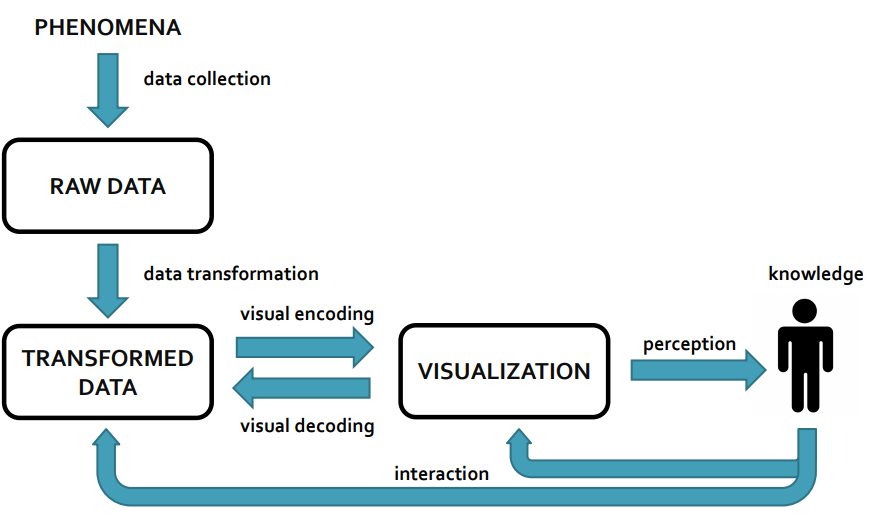
\includegraphics[width=0.5\textwidth]{images/visPipe2.png} % Sostituisci 'nome_immagine' con il nome del tuo file immagine
    \caption{Visualization pipeline}
    \label{fig:immagine}
\end{figure}
\subsection{Data}
Informazioni fattuali come misurazioni o statistiche, utilizzate come base per il ragionamento, la discussione o il calcolo.
I dati sono collezioni di \textit{items} e \textit{attributes} degli items.
Gli \textit{Items} sono gli oggetti/entità che vogliamo viusalizzare.
Gli \textit{Attributi} sono le proèrietà degli oggetti/entità.

Una \textit{Tabella} è una griaglia di colonne e righr, dove le righe  rapresentanto gli item e le colonne gli attributi.
Un \textit{network} è una collezione di nodi che rappresentano gli item, connessi tramite dei link; entrambi nodi e link possono avere attributi.

\subsection{Tipi di attributi}
\begin{itemize}
    \item \textit{Quantitativi}: sono gli attributi dove i valori rappresentano quantità misurate, 
        questi valori possono essere ordinati, ma può essere calcolata anche la distanza tra i valori.
    \item  \textit{Categorici}: sono gli attributi dove i valori descrivino le categorie,
        possono essere di tre tipi, \textbf{Nominali} se non hanno un ordine particolare, \textbf{Ordinali} se possono essere ordinati,
        \textbf{Binary} se hanno solo due stati.
\end{itemize}
\subsection{Semantica degli attributi}
\begin{itemize}
    \item \textbf{Spaziali e temporali}: Esempio la location, latitudine e longitudine o la data di assunzione come attributo temporale.
    \item \textbf{Sequnziali, ciclici divergenti}: Esempio: i mesi dell'anno sono ciclici, la temperatura è un attributo divergente.
    \item \textbf{Gerarchici}: Tipi di prodotto con sottocategorie, un esempio sono i vestiti.
\end{itemize}
Si deve selezionare la visualizzazione appropriata a seconda del tipo e dalla semantica dell'attributo.
Esempio:
\begin{figure}[H]
    \centering
    \begin{minipage}{0.45\textwidth}
        \centering
        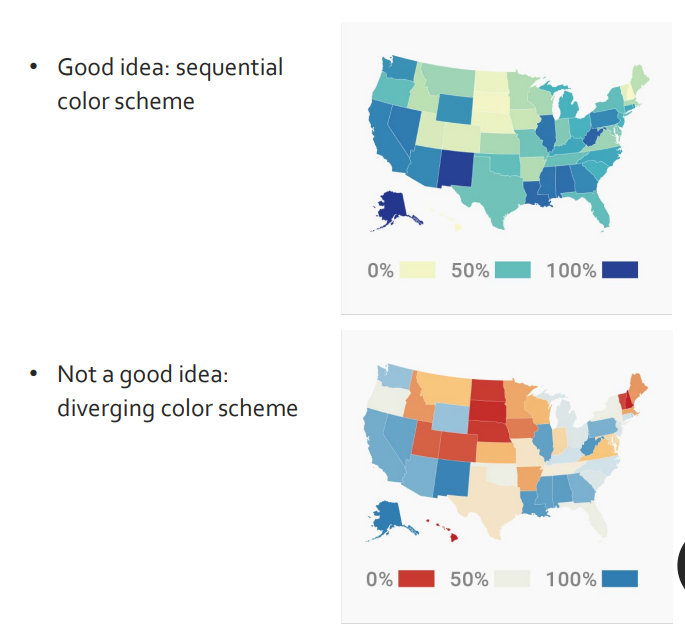
\includegraphics[width=\linewidth]{images/Attrubtevis.png} 
        \caption{Differenza di Visualizzazione}
        \label{fig:immagine1}
    \end{minipage}\hfill
    \begin{minipage}{0.45\textwidth}
        \centering
        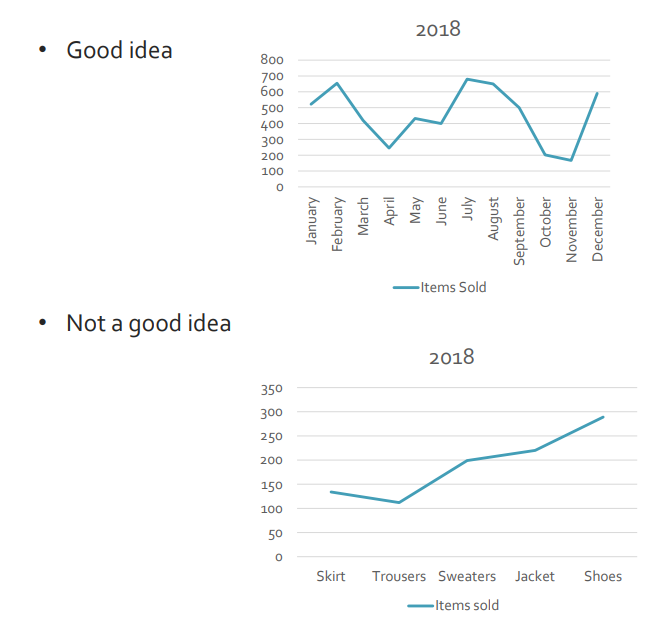
\includegraphics[width=\linewidth]{images/Attributevis2.png} % Sostituisci 'immagine2' con il nome del tuo file immagine
        \caption{Differenza di Visualizzazione}
        \label{fig:immagine2}
    \end{minipage}
\end{figure}
\subsection{Grafici Fondamentali (Bivariate data)} %--------------------------------------------------------------------------


\subsubsection{Bar Charts}
Visualizza come una quantità misurata si distribuisce tra categorie. Ogni barra rappresenta una categoria e la lunghezza della barra è una quantità misurata in quella categoria. Dati bivariati: nominale/ordinale e quantitativo.
 Non confondere con gli istogrammi
\begin{figure}[H]
    \centering
    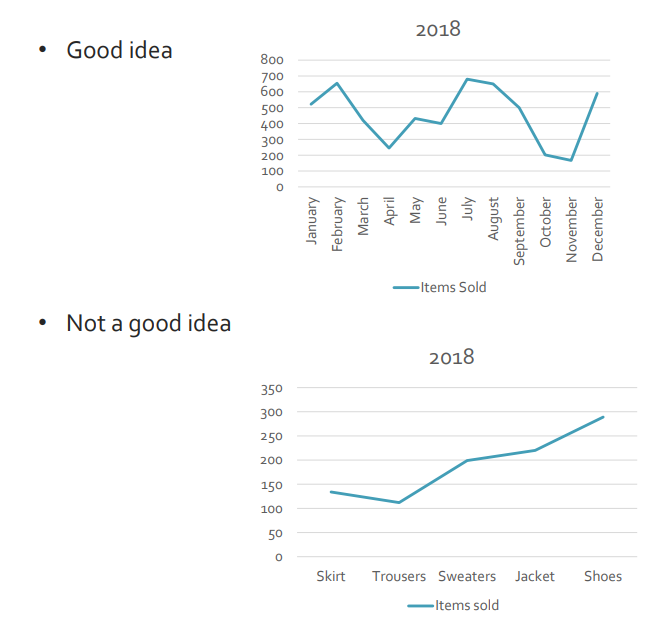
\includegraphics[width=0.5\textwidth]{images/BarCharts.png} 
    \caption{Bar Charts}
    \label{fig:immagine}
\end{figure}
\subsubsection{Histograms}
Frequenza degli elementi. Dati bivariati: una variabile indipendente quantizzata in intervalli 
(blocchi) e una variabile dipendente.
\begin{figure}[H]
    \centering
    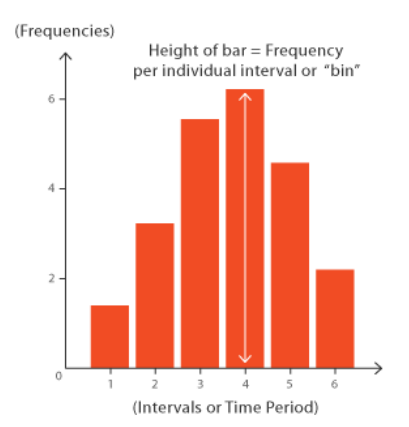
\includegraphics[width=0.5\textwidth]{images/Histograms.png} 
    \caption{Histograms}
    \label{fig:immagine}
\end{figure}
\subsubsection{Pie Charts}
Mostrare proporzioni e percentuali tra le categorie. Utile per dare un'idea rapida e confrontare una fetta rispetto al totale, non adatto per confronti accurati. Altri svantaggi: numero limitato di valori, 
occupazione dello spazio.
\begin{figure}[H]
    \centering
    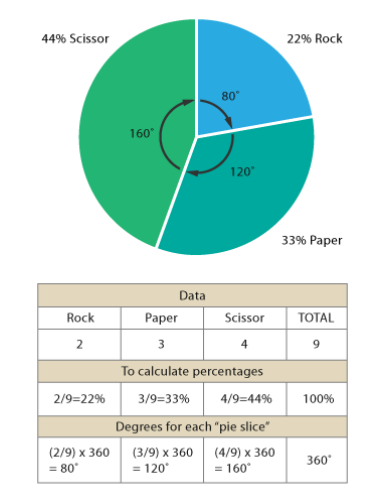
\includegraphics[width=0.5\textwidth]{images/PieChart.png} 
    \caption{Pie Charts}
    \label{fig:immagine}
\end{figure}

\subsubsection{Donut Charts}
Grafici a torta con l'area centrale tagliata. Maggiore enfasi sulla lunghezza dell'arco rispetto all'area. 
Più efficienti in termini di spazio.
\begin{figure}[H]
    \centering
    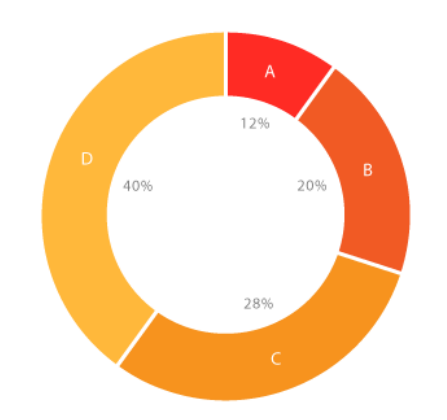
\includegraphics[width=0.5\textwidth]{images/DonutCharts.png} % Sostituisci 'nome_immagine' con il nome del tuo file immagine
    \caption{Donut Charts}
    \label{fig:immagine}
\end{figure}
\subsubsection{Scatter plots}
Relazione tra attributi: visualizzazione di come una quantità è correlata a un'altra 
(e analisi di cluster, valori anomali, ecc.). Dati bivariati: 
due attributi quantitativi indipendenti.
\begin{figure}[H]
    \centering
    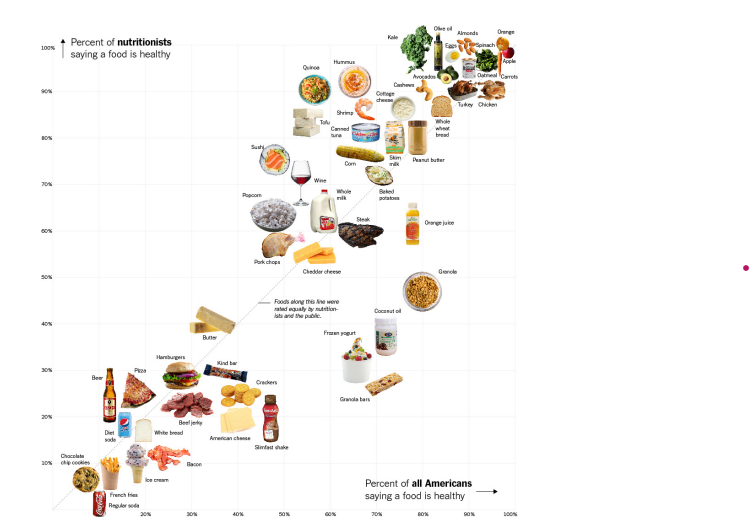
\includegraphics[width=0.5\textwidth]{images/ScatterPlots.png} % Sostituisci 'nome_immagine' con il nome del tuo file immagine
    \caption{Scatter plots}
    \label{fig:immagine}
\end{figure}
\subsubsection{Slope Charts}
Alternativa ai Scatter plots: assi paralleli, ogni elemento è una linea che collega due quantità.
\begin{figure}[H]
    \centering
    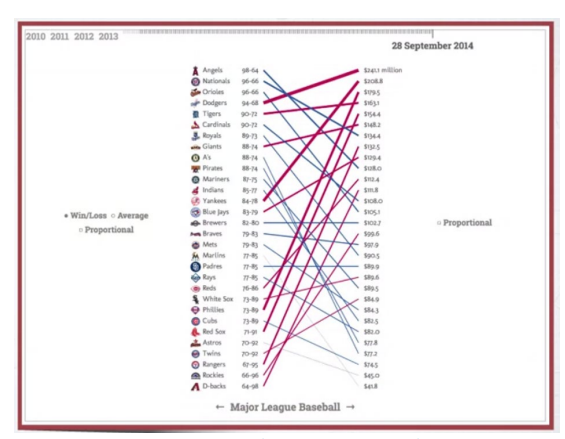
\includegraphics[width=0.5\textwidth]{images/SlopeCharts.png} 
    \caption{Slope Charts}
    \label{fig:immagine}
\end{figure}
\subsubsection{Line Charts}
\begin{figure}[H]
    \centering
    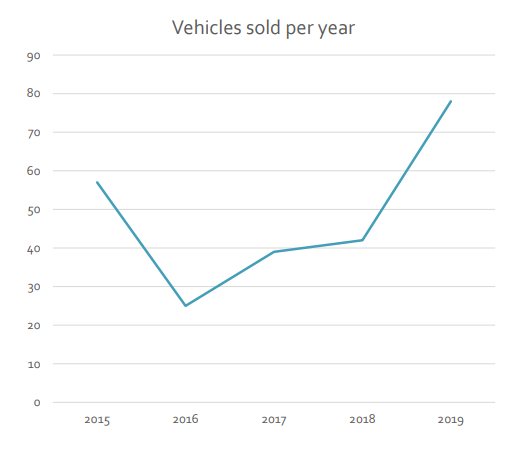
\includegraphics[width=0.5\textwidth]{images/LineCharts.png}
    \caption{Line Charts}
    \label{fig:immagine}
\end{figure}
\subsubsection{Area Charts}
Line Charts dove l'area sotto alla linea è riempita.
\begin{figure}[H]
    \centering
    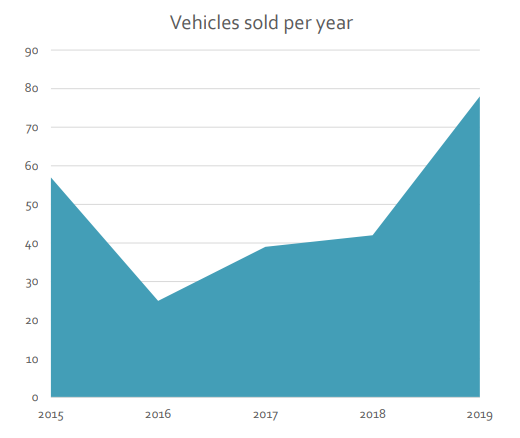
\includegraphics[width=0.5\textwidth]{images/AreaCharts.png}
    \caption{Area Charts}
    \label{fig:immagine}
\end{figure}
\subsubsection{Chropleth maps}
Come si distribuisce una quantità nelle diverse aree/geografiche/regioni. Colori, sfumature, pattern sono utilizzati per rappresentare la quantità associata alle aree/regioni. Buona panoramica (ma non confronto accurato). Rischio: 
confondere l'area geografica con i valori dei dati (prestare attenzione alla normalizzazione).
\begin{figure}[H]
    \centering
    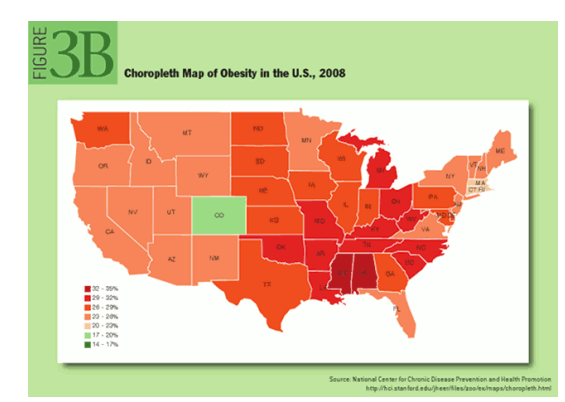
\includegraphics[width=0.5\textwidth]{images/Chropolet.png} 
    \caption{Chropleth maps}
    \label{fig:immagine}
\end{figure}
\subsubsection{Symbol maps}
Come si distribuisce una quantità lungo due coordinate spaziali. Un simbolo (spesso un disco o un quadrato) è posizionato 
in un punto e dimensionato in modo che la sua area sia proporzionale alla quantità associata al punto.
\begin{figure}[H]
    \centering
    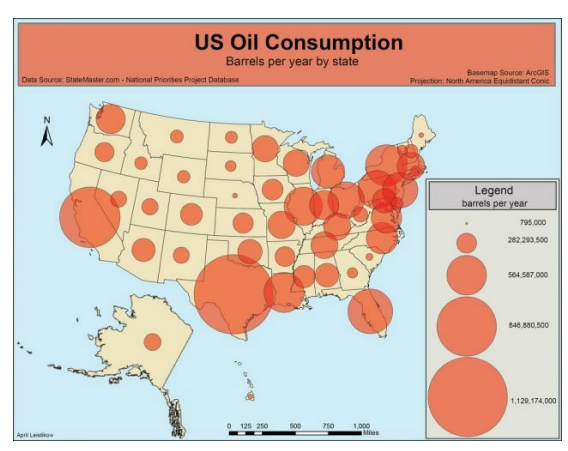
\includegraphics[width=0.5\textwidth]{images/SymbolMaps.png} 
    \caption{Symbol maps}
    \label{fig:immagine}
\end{figure}

\subsection{Grafici Fondamentali (Attributi Multipli)}
\subsubsection{Stacked Bar Charts}
\begin{figure}[H]
    \centering
    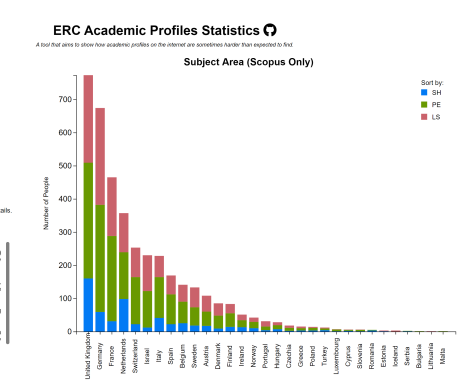
\includegraphics[width=0.5\textwidth]{images/StackedBar.png} % Sostituisci 'nome_immagine' con il nome del tuo file immagine
    \caption{Stacked Bar Charts}
    \label{fig:immagine}
\end{figure}
\subsubsection{Grouped Bar Charts}
\begin{figure}[H]
    \centering
    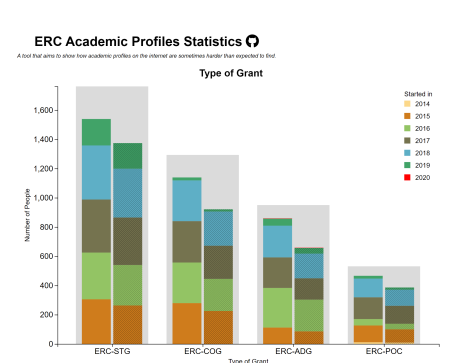
\includegraphics[width=0.5\textwidth]{images/GroupedBar.png} % Sostituisci 'nome_immagine' con il nome del tuo file immagine
    \caption{Grouped Bar Charts}
    \label{fig:immagine}
\end{figure}
\subsubsection{Stacked Line Charts}
\begin{figure}[H]
    \centering
    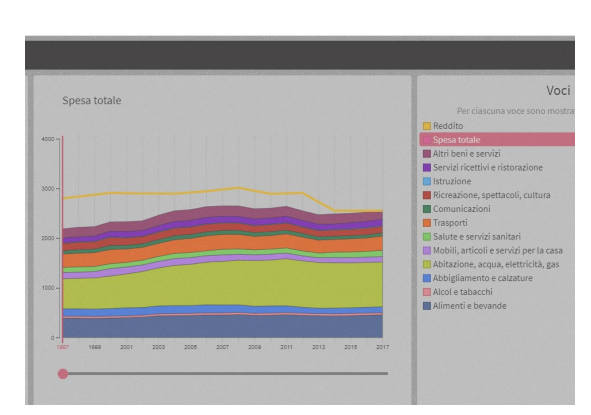
\includegraphics[width=0.5\textwidth]{images/Stacked.png} % Sostituisci 'nome_immagine' con il nome del tuo file immagine
    \caption{Stacked Line Charts}
    \label{fig:immagine}
\end{figure}
\subsubsection{Line Charts Series}
\begin{figure}[H]
    \centering
    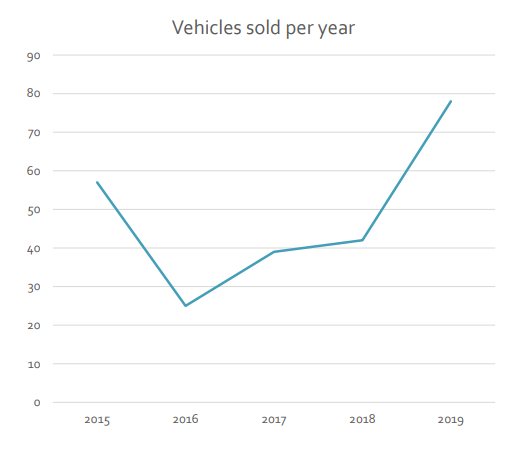
\includegraphics[width=0.5\textwidth]{images/LineCharts.png} % Sostituisci 'nome_immagine' con il nome del tuo file immagine
    \caption{Line Charts Series}
    \label{fig:immagine}
\end{figure}
\subsubsection{Bubble Charts}
\begin{figure}[H]
    \centering
    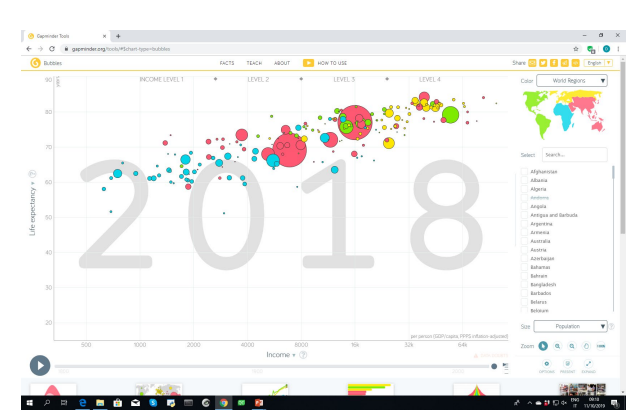
\includegraphics[width=0.5\textwidth]{images/Bubble.png} % Sostituisci 'nome_immagine' con il nome del tuo file immagine
    \caption{Bubble Charts}
    \label{fig:immagine}
\end{figure}
\subsubsection{Small multiples}
\begin{figure}[H]
    \centering
    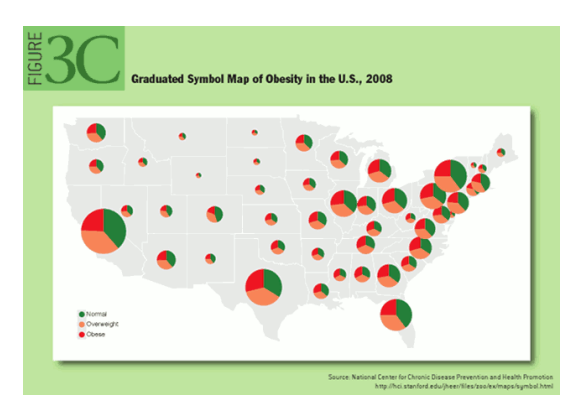
\includegraphics[width=0.5\textwidth]{images/SmallMultiples2.png} % Sostituisci 'nome_immagine' con il nome del tuo file immagine
    \caption{Small multiples}
    \label{fig:immagine}
\end{figure}
\subsubsection{Symbol Maps}
\begin{figure}[H]
    \centering
    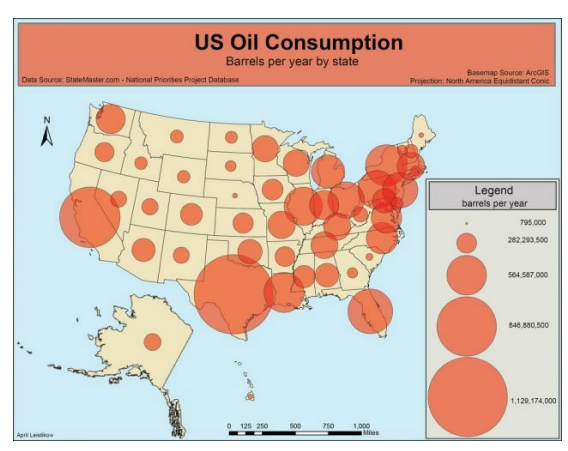
\includegraphics[width=0.5\textwidth]{images/SymbolMaps.png} % Sostituisci 'nome_immagine' con il nome del tuo file immagine
    \caption{Symbol Maps}
    \label{fig:immagine}
\end{figure}
\subsection{Grafici Fondamentali (Attributi Gerarchici)}
\subsubsection{Sunburst Charts}
\begin{figure}[H]
    \centering
    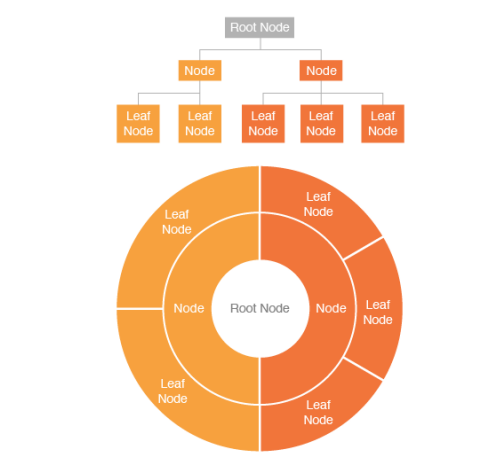
\includegraphics[width=0.5\textwidth]{images/SunBurst.png} % Sostituisci 'nome_immagine' con il nome del tuo file immagine
    \caption{Sunburst Charts}
    \label{fig:immagine}
\end{figure}
\subsubsection{Treempas}
\begin{figure}[H]
    \centering
    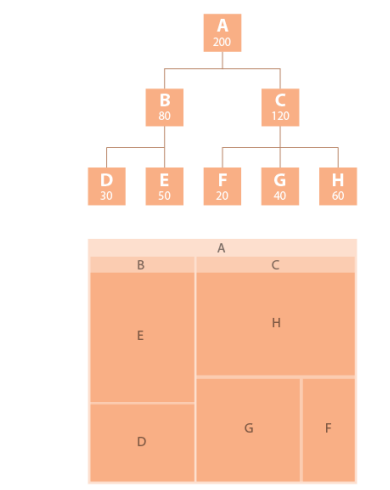
\includegraphics[width=0.5\textwidth]{images/TreeMpas.png} % Sostituisci 'nome_immagine' con il nome del tuo file immagine
    \caption{Treempas}
    \label{fig:immagine}
\end{figure}